\section{Comparativa y Benchmarks}

\begin{frame}{Rendimiento y sobrecarga}
  \small
  \begin{tabular}{@{}L{0.35\textwidth}L{0.28\textwidth}L{0.28\textwidth}@{}}
    \toprule
    & \textbf{C/OpenMP} & \textbf{Python (multiprocessing)} \\
    \midrule
    Rendimiento CPU & Base 1.0x; acceso directo a registros & 0.1x--0.5x limitado por pickle e IPC \\
    Threading CPU & Paralelo real & Serializado por GIL \\
    Tiempo de inicio & Microsegundos (hilos ligeros) & Milisegundos (procesos) \\
    Memoria & Compartida, requiere sincronización & Copia de heap; memoria aislada \\
    Comunicación & Punteros, cero copia & Pickle por tuberías o sockets \\
    \bottomrule
  \end{tabular}
\end{frame}

\begin{frame}{Costo de desarrollo vs. ejecución}
  \begin{itemize}
    \item C/OpenMP: mayor esfuerzo de depuración y manejo de memoria; ideal para rutas críticas que se ejecutan millones de veces.
    \item Python/Joblib: itera rápido y simplifica pipelines; aceptable cuando el tiempo de pared no es crítico.
    \item Estrategia híbrida: usar Python como orquestador y bajar a extensiones en C o Numba cuando el perfil marque cuellos de botella.
  \end{itemize}
\end{frame}

\begin{frame}{Arquitectura híbrida recomendada}
  \begin{itemize}
    \item Núcleo de cómputo intensivo en C/C++ u OpenMP, liberando el GIL y aprovechando NUMA.
    \item Capa de orquestación y análisis en Python con Joblib, NumPy o Numba.
    \item Integración por FFI, extensiones o bindings para mantener un solo pipeline de entrega.
  \end{itemize}
  \begin{figure}
    \centering
    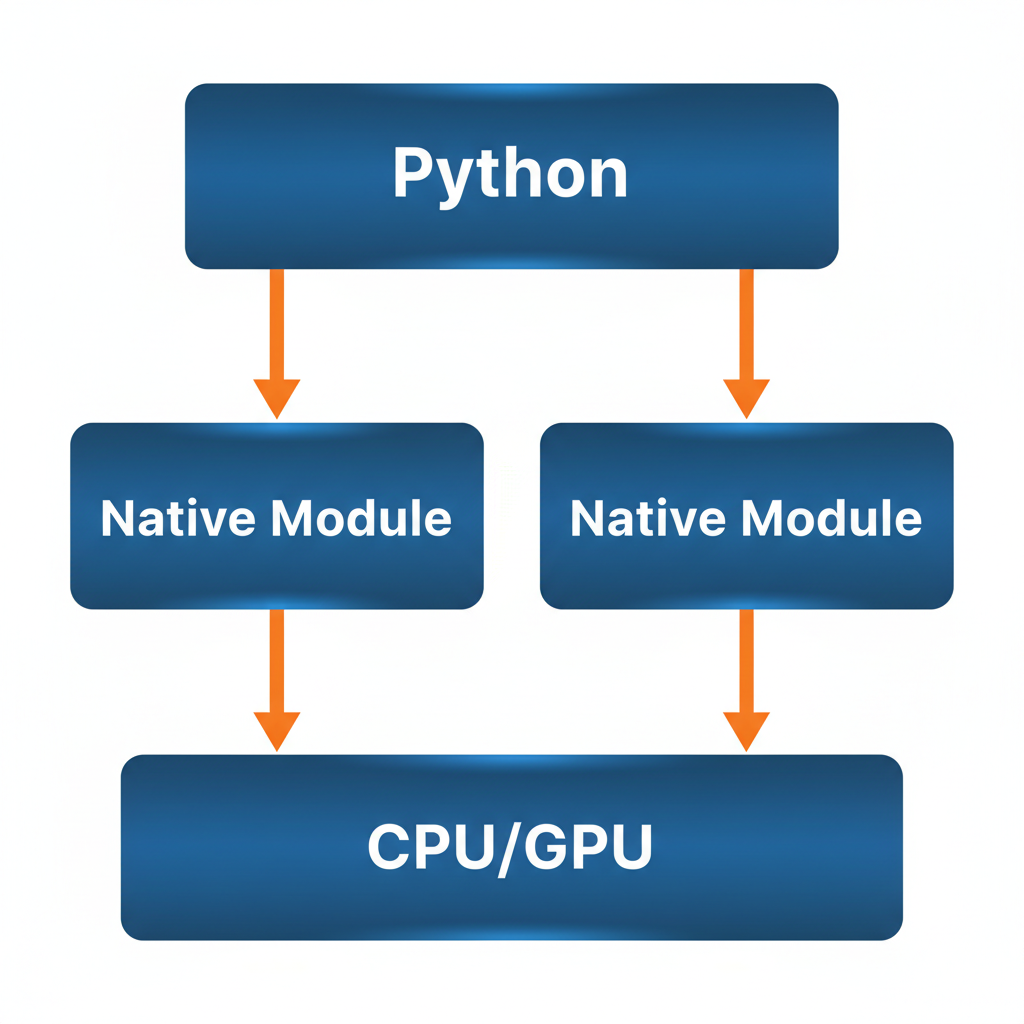
\includegraphics[height=0.45\textheight]{img/06-arquitectura-hibrida.png}
    \caption{Arquitectura híbrida con Python como orquestador.}
  \end{figure}
\end{frame}
